\subsection{Courses}\vspace{-0.2cm}
The PhD degree requires 75 ECTS from the courses credit which is met as shown in Table \ref{tbl_courses}.
\vspace{-0.2cm}
\begin{table}[h]
	\renewcommand{\arraystretch}{1.3}
	\begin{tabularx}{\textwidth}{|X|p{15mm}|p{18mm}|}
		\hline \rowcolor{gray!10}
		\textbf{Courses} & \centering\arraybackslash \textbf{Credits} & \centering\arraybackslash \textbf{Status} \\
		\hline
		Individual Project & \centering\arraybackslash7.5 & \centering\arraybackslash Finished \\
		\hline
		VeriSpec Project: ReSA Toolchain Integration into AREATOP IDE, VGTT & \centering\arraybackslash7.5 & \centering\arraybackslash Finished \\
		\hline
        Advanced Component-based Software Engineering & \centering\arraybackslash7.5 & \centering\arraybackslash Finished \\
		\hline
		Research Planning & \centering\arraybackslash4.5 & \centering\arraybackslash Finished \\
		\hline
		Research Methods & \centering\arraybackslash7.5 & \centering\arraybackslash Finished \\
		\hline
		Advanced Validation and Verification  & \centering\arraybackslash7.5 & \centering\arraybackslash Finished \\
		\hline
		Principles of Cyber-physical Systems  & \centering\arraybackslash7.5 & \centering\arraybackslash Finished \\
		\hline
		Safety Critical Systems Engineering  & \centering\arraybackslash7.5 & \centering\arraybackslash Finished \\
		\hline
		Project Management and research commercialization  & \centering\arraybackslash 7.5 & \centering\arraybackslash Finished \\
		\hline
	  %  Introduction to Graduate Education for new PhD students  & \centering\arraybackslash 4.5 & \centering\arraybackslash Finished \\
	%	\hline
	    Industrial Systems Cloud Computing  & \centering\arraybackslash7.5 & \centering\arraybackslash Finished \\
		\hline
        International Summer School Marktoberdorf, July 29 to August 10, 2014 & \centering\arraybackslash3.0 & \centering\arraybackslash Finished\\
        \hline
      %  Fourth Summer School on Formal Techniques May 19 - May 23, 2014 Menlo College, Atherton, CA &\centering\arraybackslash2.0 & \centering\arraybackslash Finished\\
        %\hline
       % PhD visit &\centering\arraybackslash 1.0 & \centering\arraybackslash Finished\\
      %  \hline
		\textbf{Total Credits} & \centering\arraybackslash \textbf{75} & \\
		\hline
	\end{tabularx}
	
	\caption{List of Courses Taken.}\vspace{-0.2cm}
		\label{tbl_courses}
\label{coursestble}
\end{table}

\subsection{Time Plan}\vspace{-0.2cm}
The time plan from the beginning of October to the time the PhD thesis is defended is shown as follows:\\[6pt]
 %\tikzset{png export}
\resizebox{1\textwidth}{!}{

    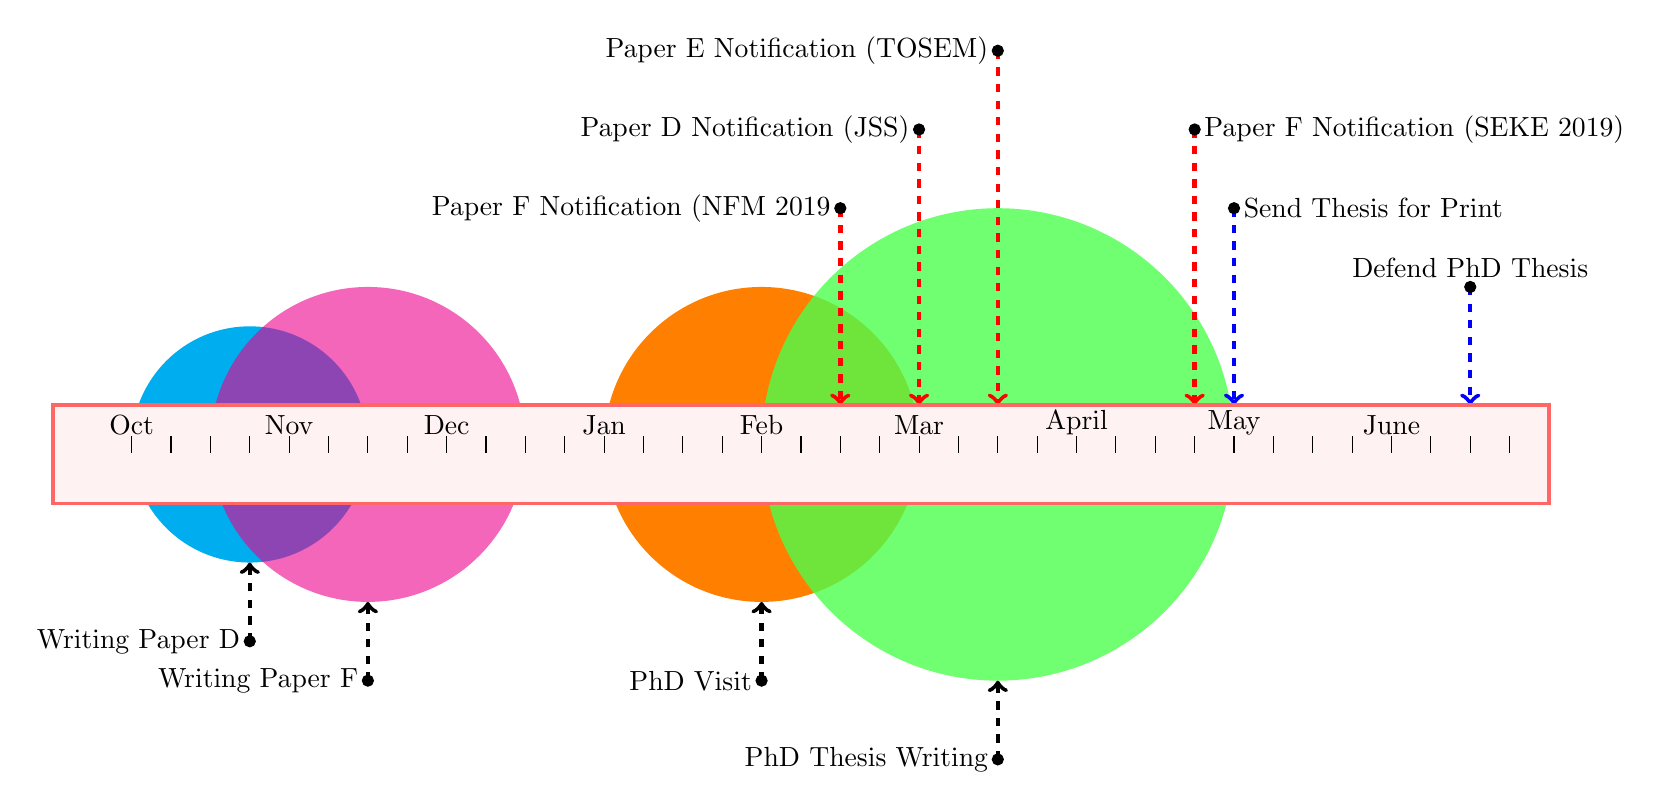
\begin{tikzpicture}
    
    \def\totalmonths{9}
    \def\timelinewidth{18}
    \pgfmathsetmacro\tunit{\timelinewidth/\totalmonths}
    
    % Paper F
    \def\wkPE{8}% working weeks
    \def\offPE{2}
    \def\wkPES{6}% submission week
    \def\wkPEN{16}% notification week
    
    % Paper D
    \def\wkPG{6}% working weeks
    \def\offPG{0}
    \def\wkPGS{8}% submission week
    \def\wkPGN{10}% notification week
    
    % Paper E
    \def\wkPDN{5}% notification week
    
    \def\wkVisit{8}% number of weeks
    \def\wkVisitOff{12}% number of weeks
    \def\wkThesis{12}% number of weeks
    \def\wkThesisOff{16}% number of weeks

    \newcommand{\fWk}[1]
    {
      { #1*\scl}
    }
    \newcommand{\calcx}[2]
    {
      { #1*\tunit + #2*\tunit/4}
    }
    \newcommand{\radius}[1]
    {
      {#1*\tunit/2/4}
    }
    \newcommand{\offset}[2]
    {
      {#1*\tunit/4 + #2}
    }
    \newcommand{\legend}[3]
    {
      { 
         \draw[color=black, dash pattern=on 3pt off 3pt, ultra thick, ->] ({#1},-\radius{#2}-1, 0) -- ({#1},{-\radius{#2}});
         \filldraw[black] ({#1},{-\radius{#2}-1}) circle (2pt) node[anchor=east] {#3};
      }
    }
    \newcommand{\legendNotification}[5]%
    {
      { 
        \draw[color=red, dash pattern=on 3pt off 3pt, ultra thick, ->] ({#1},{#2+#3}, 0) -- ({#1},{#2+0.5});
         \filldraw[black] ({#1},{#2+#3}) circle (2pt) node[anchor=#5] {#4};
      }
    }
    \newcommand{\legendSubmission}[5]%
    {
      { 
        \draw[color=blue, dash pattern=on 3pt off 3pt, ultra thick, ->] ({#1},{#2+#3}, 0) -- ({#1},{#2+0.5});
         \filldraw[black] ({#1},{#2+#3}) circle (2pt) node[anchor=#5] {#4};
      }
    }
          
   
   
    % Paper D
   \fill[fill=cyan](\offset{\offPG}{\wkPG/4},0) circle (\radius{\wkPG});
   \legend{\offset{\offPG}{\wkPG/4}}{\wkPG}{Writing Paper D};
   
   
   % Paper F
    \fill[fill=magenta, fill opacity=0.6](\offset{\offPE}{\wkPE/4},0) circle (\radius{\wkPE}); 
    %\fill[fill=magenta, fill opacity=0.6](0,0) circle (\radius{\wkPE}); 
    \legend{\offset{\offPE}{\wkPE/4}}{\wkPE}{Writing Paper F};

    % Phd visit
    %\draw[pattern=dots, pattern
    \fill[fill=orange](\offset{\wkVisitOff}{\wkVisit/4}, 0) circle (\radius{\wkVisit});
   \legend{\offset{\wkVisitOff}{\wkVisit/4}}{\wkVisit}{PhD Visit};


   % Thesis writing
    %\draw[pattern=dots, pattern
    \fill[fill=green!70,fill opacity=0.8](\offset{\wkThesisOff}{\wkThesis/4}, 0) circle (\radius{\wkThesis});
    \legend{\offset{\wkThesisOff}{\wkThesis/4}}{\wkThesis}{PhD Thesis Writing};


    %% Notifications
    \legendNotification{\offset{18}{0}}{0}{3}{Paper F Notification (NFM 2019}{east};%(x,y,height, message)
    \legendNotification{\offset{20}{0}}{0}{4}{Paper D Notification (JSS)}{east};
    \legendNotification{\offset{22}{0}}{0}{5}{Paper E Notification (TOSEM)}{east};
    \legendSubmission{\offset{28}{0}}{0}{3}{Send Thesis for Print}{west};
    \legendNotification{\offset{27}{0}}{0}{4}{Paper F Notification (SEKE 2019)}{west};
    \legendSubmission{\offset{34}{0}}{0}{2}{Defend PhD Thesis}{south};
    
    % Draw timeline
    \filldraw[color=red!60, fill=red!5, very thick] (-1,-0.75) rectangle (\timelinewidth,0.5);
    \foreach \x/\y in {0/Oct,1/Nov,2/Dec,3/Jan,4/Feb,5/Mar,6/April,7/May,8/June }
    {       
        \draw (\calcx{\x}{0},3pt) -- (\calcx{\x}{0},-3pt) node[above=3pt] {\y}; 
        \foreach \z in {1,2,3} 
           \draw (\calcx{\x}{\z},3pt) -- (\calcx{\x}{\z},-3pt);
    }
    % \pgfmathsetmacro\resultt{(\j * 2) + 1}
  \end{tikzpicture}}
%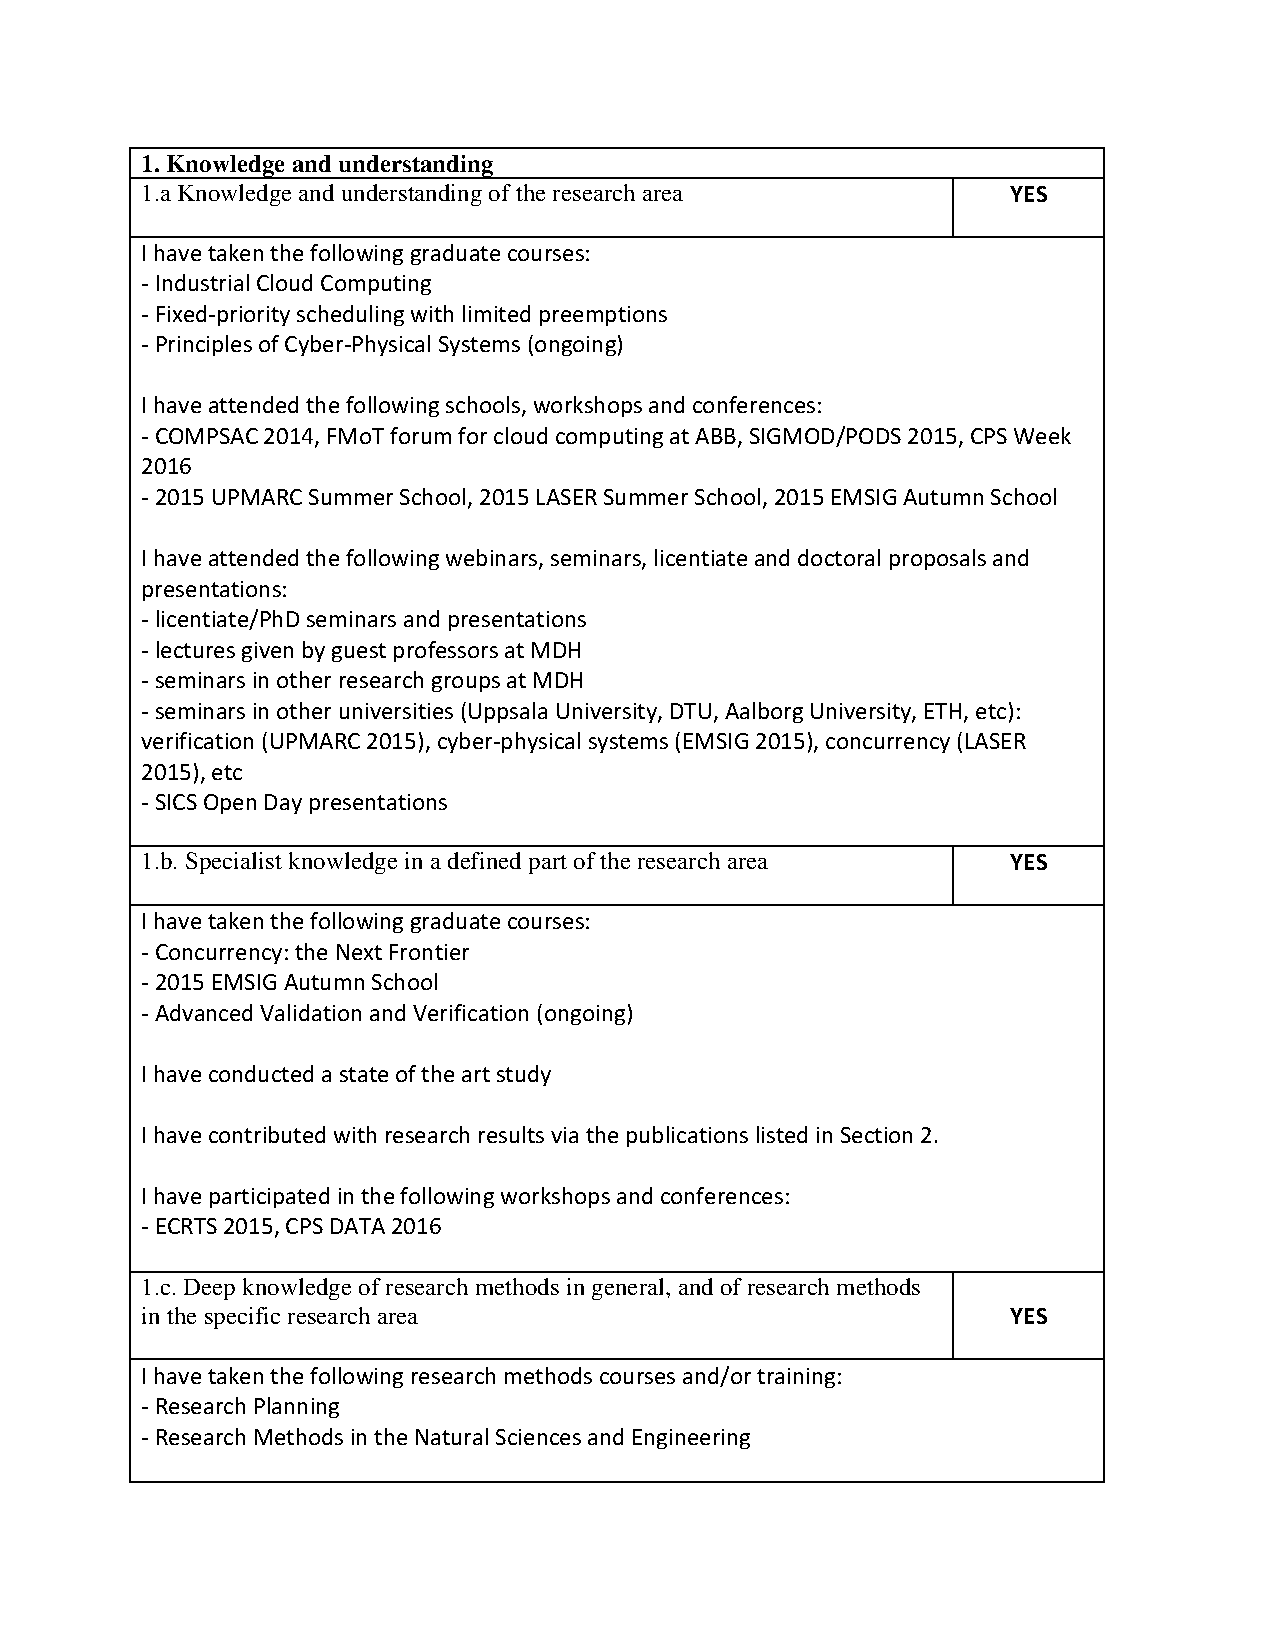
\includepdf[pages=-]{thirdcycle.pdf}
\pagebreak

%research area
\subsection{Thesis Opponent and Committee}
For the thesis defense we propose the preliminary committee as follows:
\begin{enumerate}
	\item Opponent: Prof. Joost-Pieter Katoen, RWTH Aachen University, Germany, and University of Twente, the Netherlands
	\item Committee members:
	\begin{enumerate}
		\item Antonia Bertolino, Research Director at CNR, Italy
		\item Associate Professor Patrizio Pellicione, Chalmers University of Technology, Sweden
        \item Professor Peter Csaba {\"0}lveczky, University of Oslo, Norway
      %  \item Professor Einar Broch Johnsen, University of Oslo, Norway
		%\item Assistant Professor Marco Autili, University of  L'Aquila, Italy
	\end{enumerate}
	\item Reserve: To be decided
\end{enumerate}